\documentclass[9pt,sans-serif]{beamer}
\usepackage{amsmath}
\usepackage{concrete}
\usetheme{Madrid}
\usecolortheme{rose}
\usefonttheme{structuresmallcapsserif}
\usepackage{bookman}

\title[Discrete Morse Theory]{Discrete Morse Theory and Applications}

\author[Sush]{Sushovan ``\textcolor{magenta}{Sush}'' MAJHI} \date[Tulane
  University '18]{Topology and Geometry Seminar \\ Tulane University, 2018}

\begin{document}
\frame{\titlepage}


\begin{frame}{Myself}
  I am a fifth year PhD student at Tulane University.
  \\
  \pause
  \vspace{50pt}
  \textbf{My Collaborators:}\\
  \textcolor{blue}{Carola Wenk}, Computer Science, Tulane University\\
  \textcolor{blue}{Rafal Komendarczyk}, Mathematics, Tulane University \\
  \textcolor{blue}{Brittany Terese Fasy}, Computer Science, Montana State University \\
  \textcolor{blue}{Yusu Wang}, Computer Science, Ohio State University
\end{frame}

\begin{frame}{Classical Morse Theory}
  \begin{block}{Motivation}
    A reasonably "good'' smooth function reveals the
    \textcolor{blue}{Combinatorial Description} of a smooth manifold.
  \end{block}
\end{frame}

\begin{frame}{Classical Morse Theory}
  Let $M^n$ be a smooth manifold and $f:M\to\mathbb R$ be a smooth function. 
  
  \begin{block}{Critical Point}
    A point $p\in M$ is called a \textcolor{blue}{critical point} of $f$ if
    $Df=0$.
    
    \pause
    \vspace{10pt}
    
    A critical point $p$ is \textcolor{magenta}{non-degenerate} if $Hess(f)$ is
    non-singular. \\
    The number of -ve eigen values if called the \textcolor{red}{index} of $p$.
  \end{block}
  
  
  \pause
  
  \begin{figure}
    \centering
    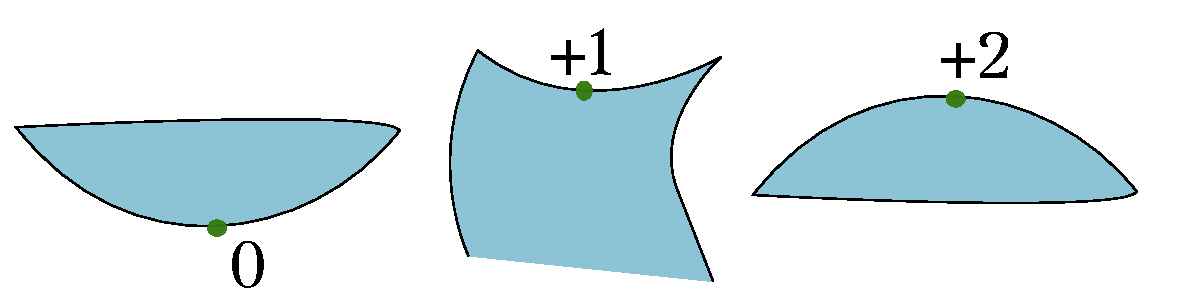
\includegraphics[scale=0.5]{critical}
    \caption{critical points with index}
  \end{figure}

\end{frame}

\begin{frame}{Classical Morse Theory}  
  \begin{block}{Morse Function}
    A smooth function $f:M^n\to\mathbb R$ is called a \textcolor{blue}{Morse
      function} if all its critical points are non-degenerate.  \\ \pause

    $p$ has index \textcolor{magenta}{0}. $w$ has index
    \textcolor{magenta}{+2}. Others have index \textcolor{magenta}{+1}.

  \end{block}
  
  
  \begin{figure}
    \centering
    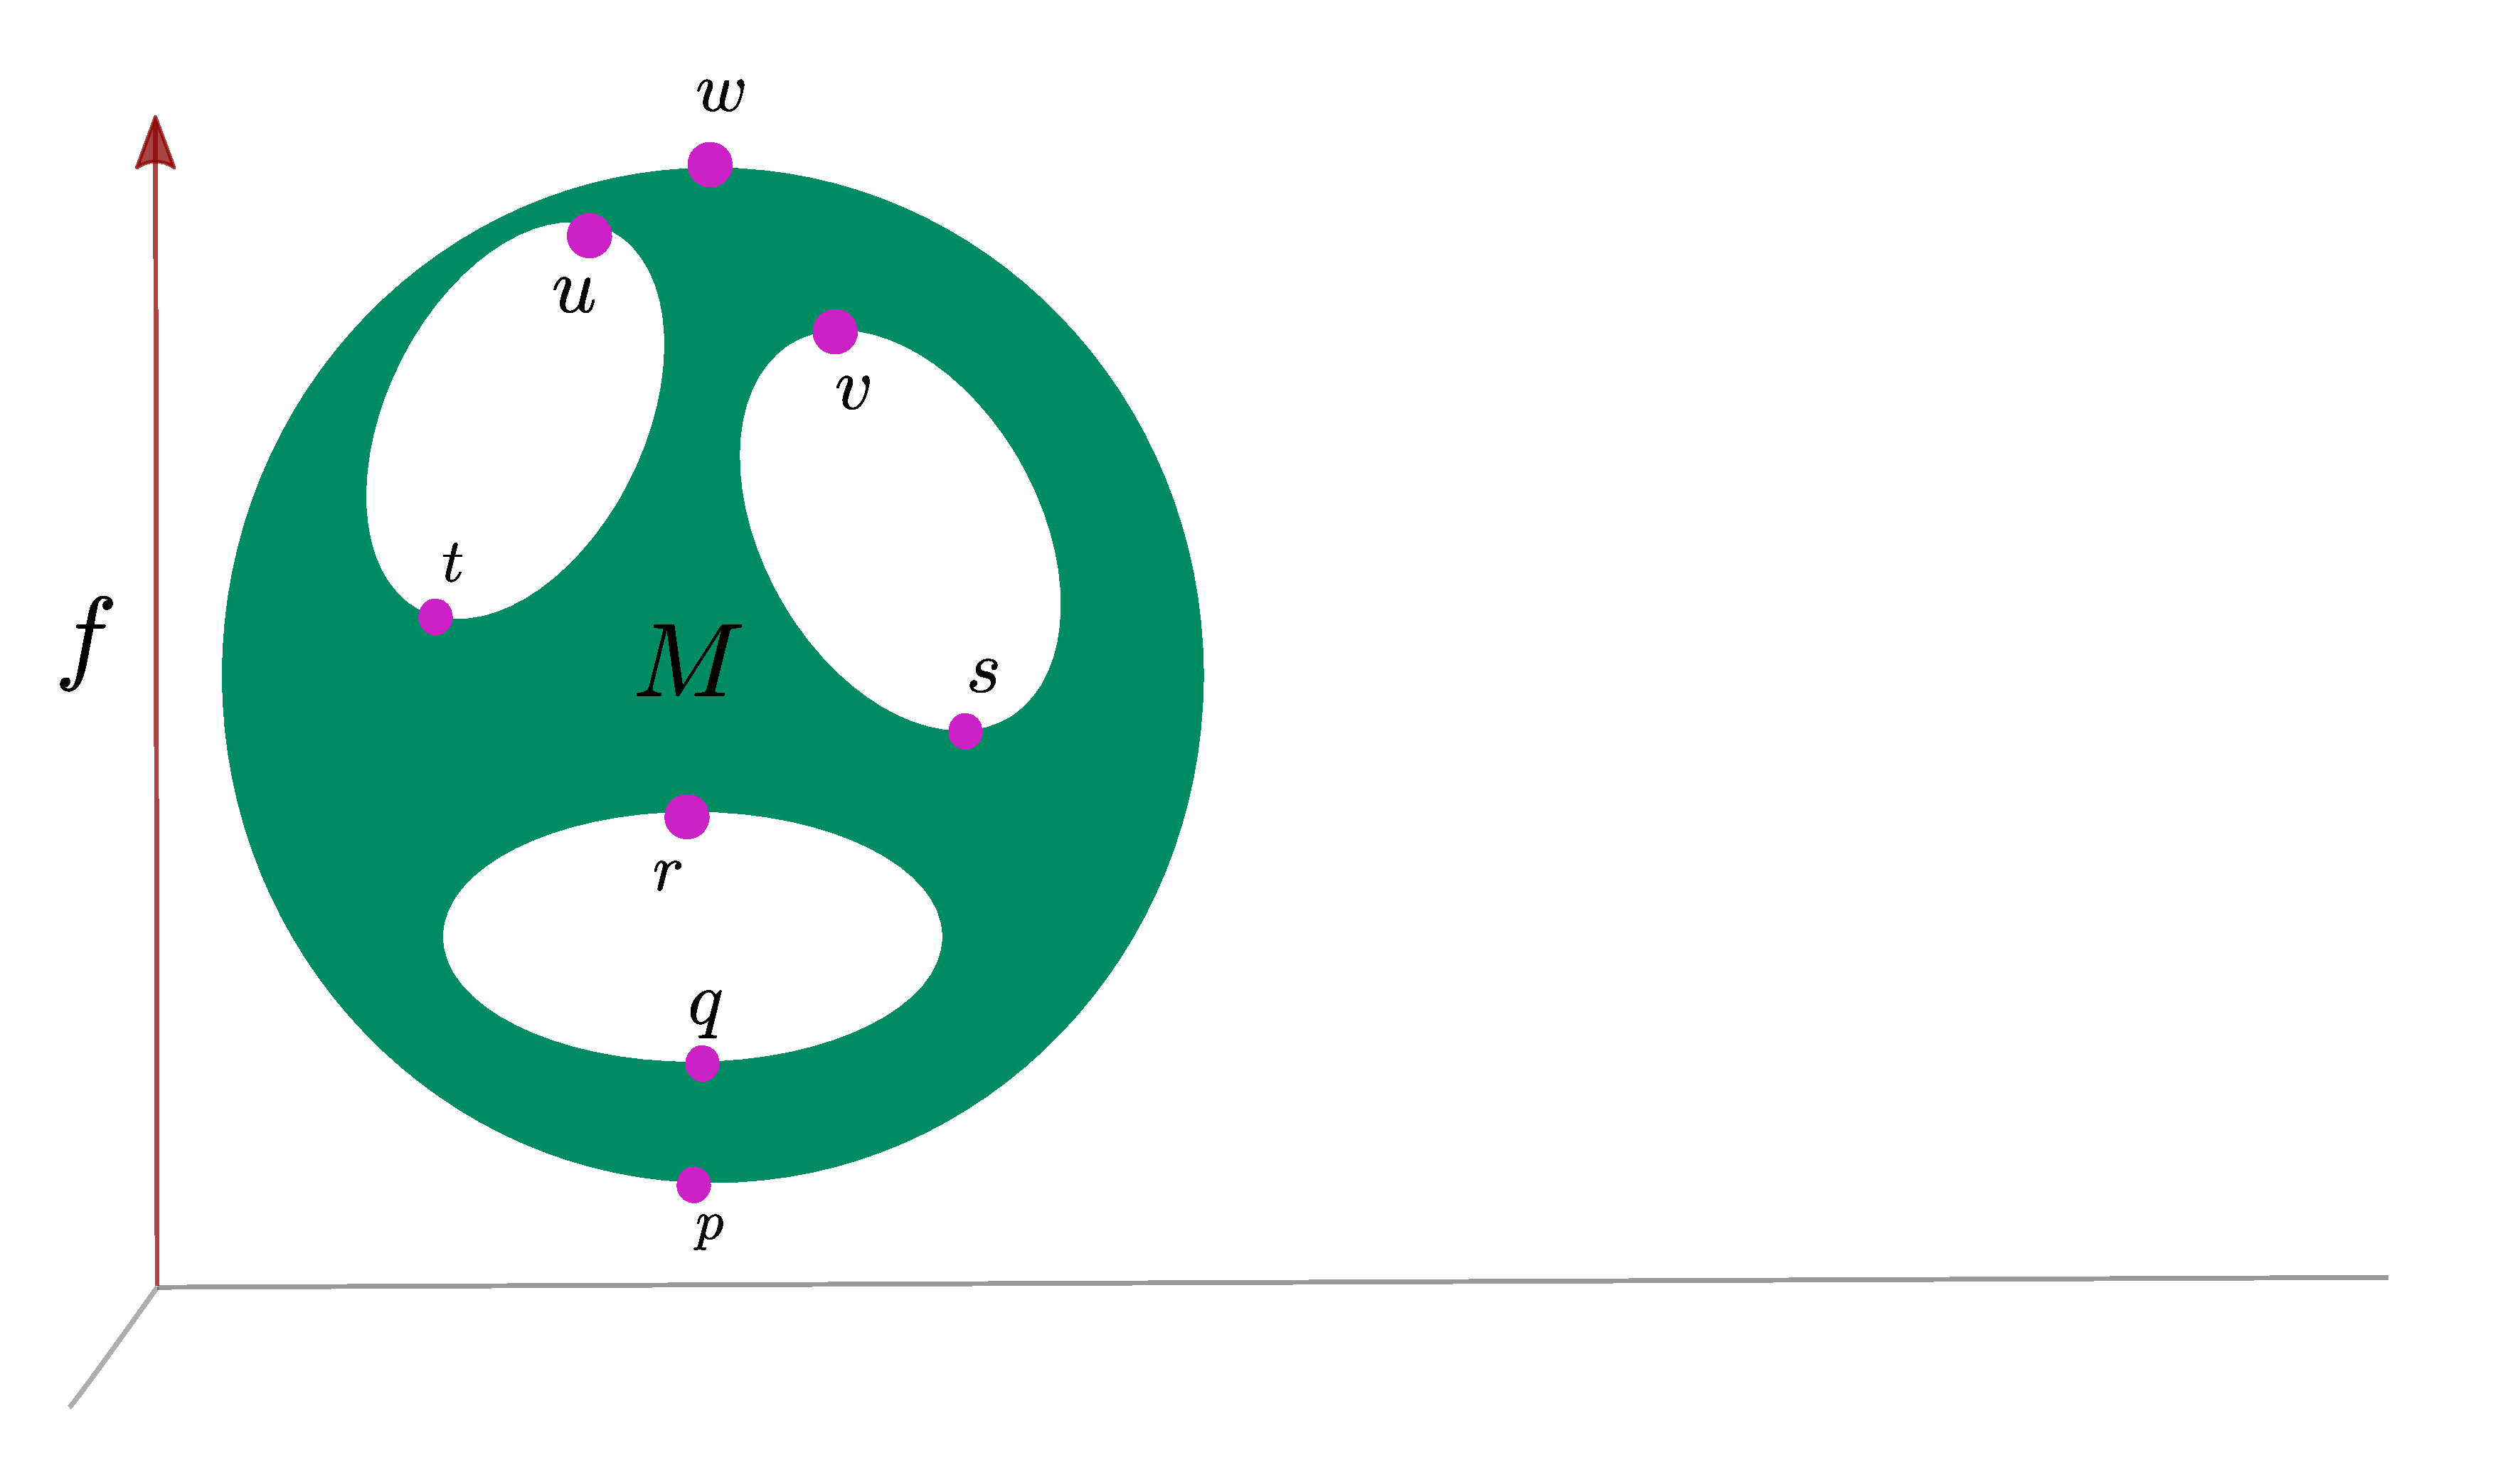
\includegraphics[scale=0.15]{0}
    \caption{Morse Function}
  \end{figure}

\end{frame}


\begin{frame}{Classical Morse Theory}
  \begin{figure}
    \centering
    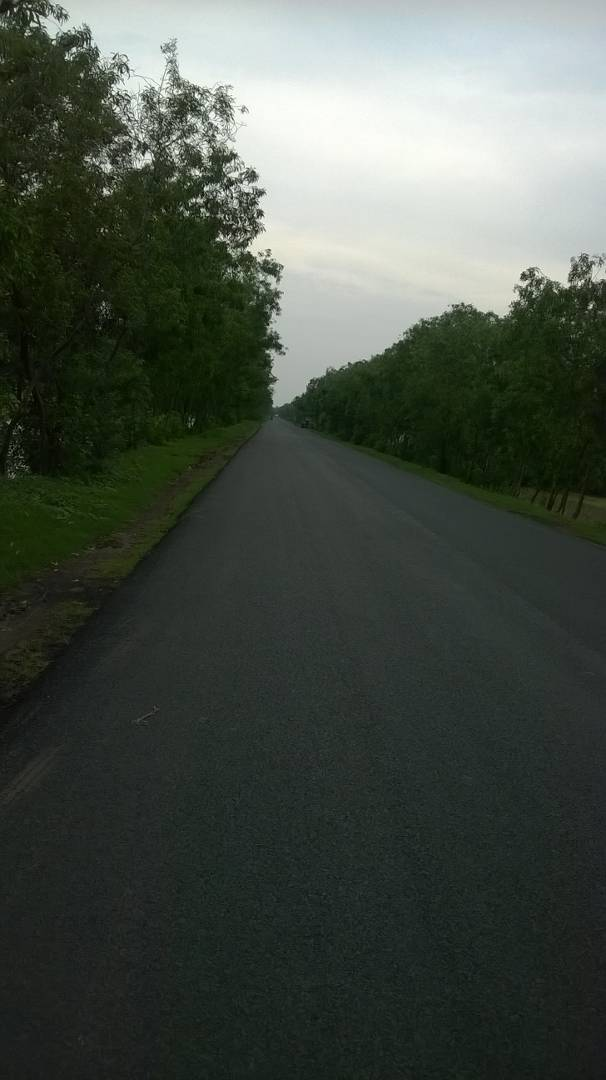
\includegraphics[scale=0.2]{1}
    \caption{Sub-level Set}
  \end{figure}
\end{frame}

\begin{frame}{Classical Morse Theory}  
  \begin{figure}
    \centering
    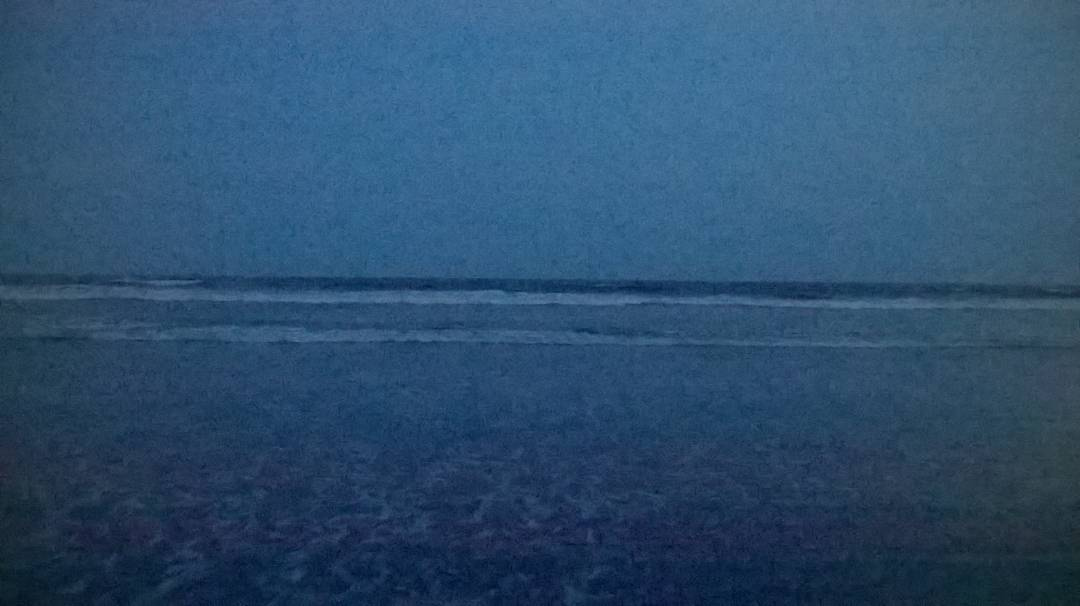
\includegraphics[scale=0.2]{2}
    \caption{Sub-level Set}
  \end{figure}
\end{frame}

\begin{frame}{Classical Morse Theory}
  \begin{figure}
    \centering
    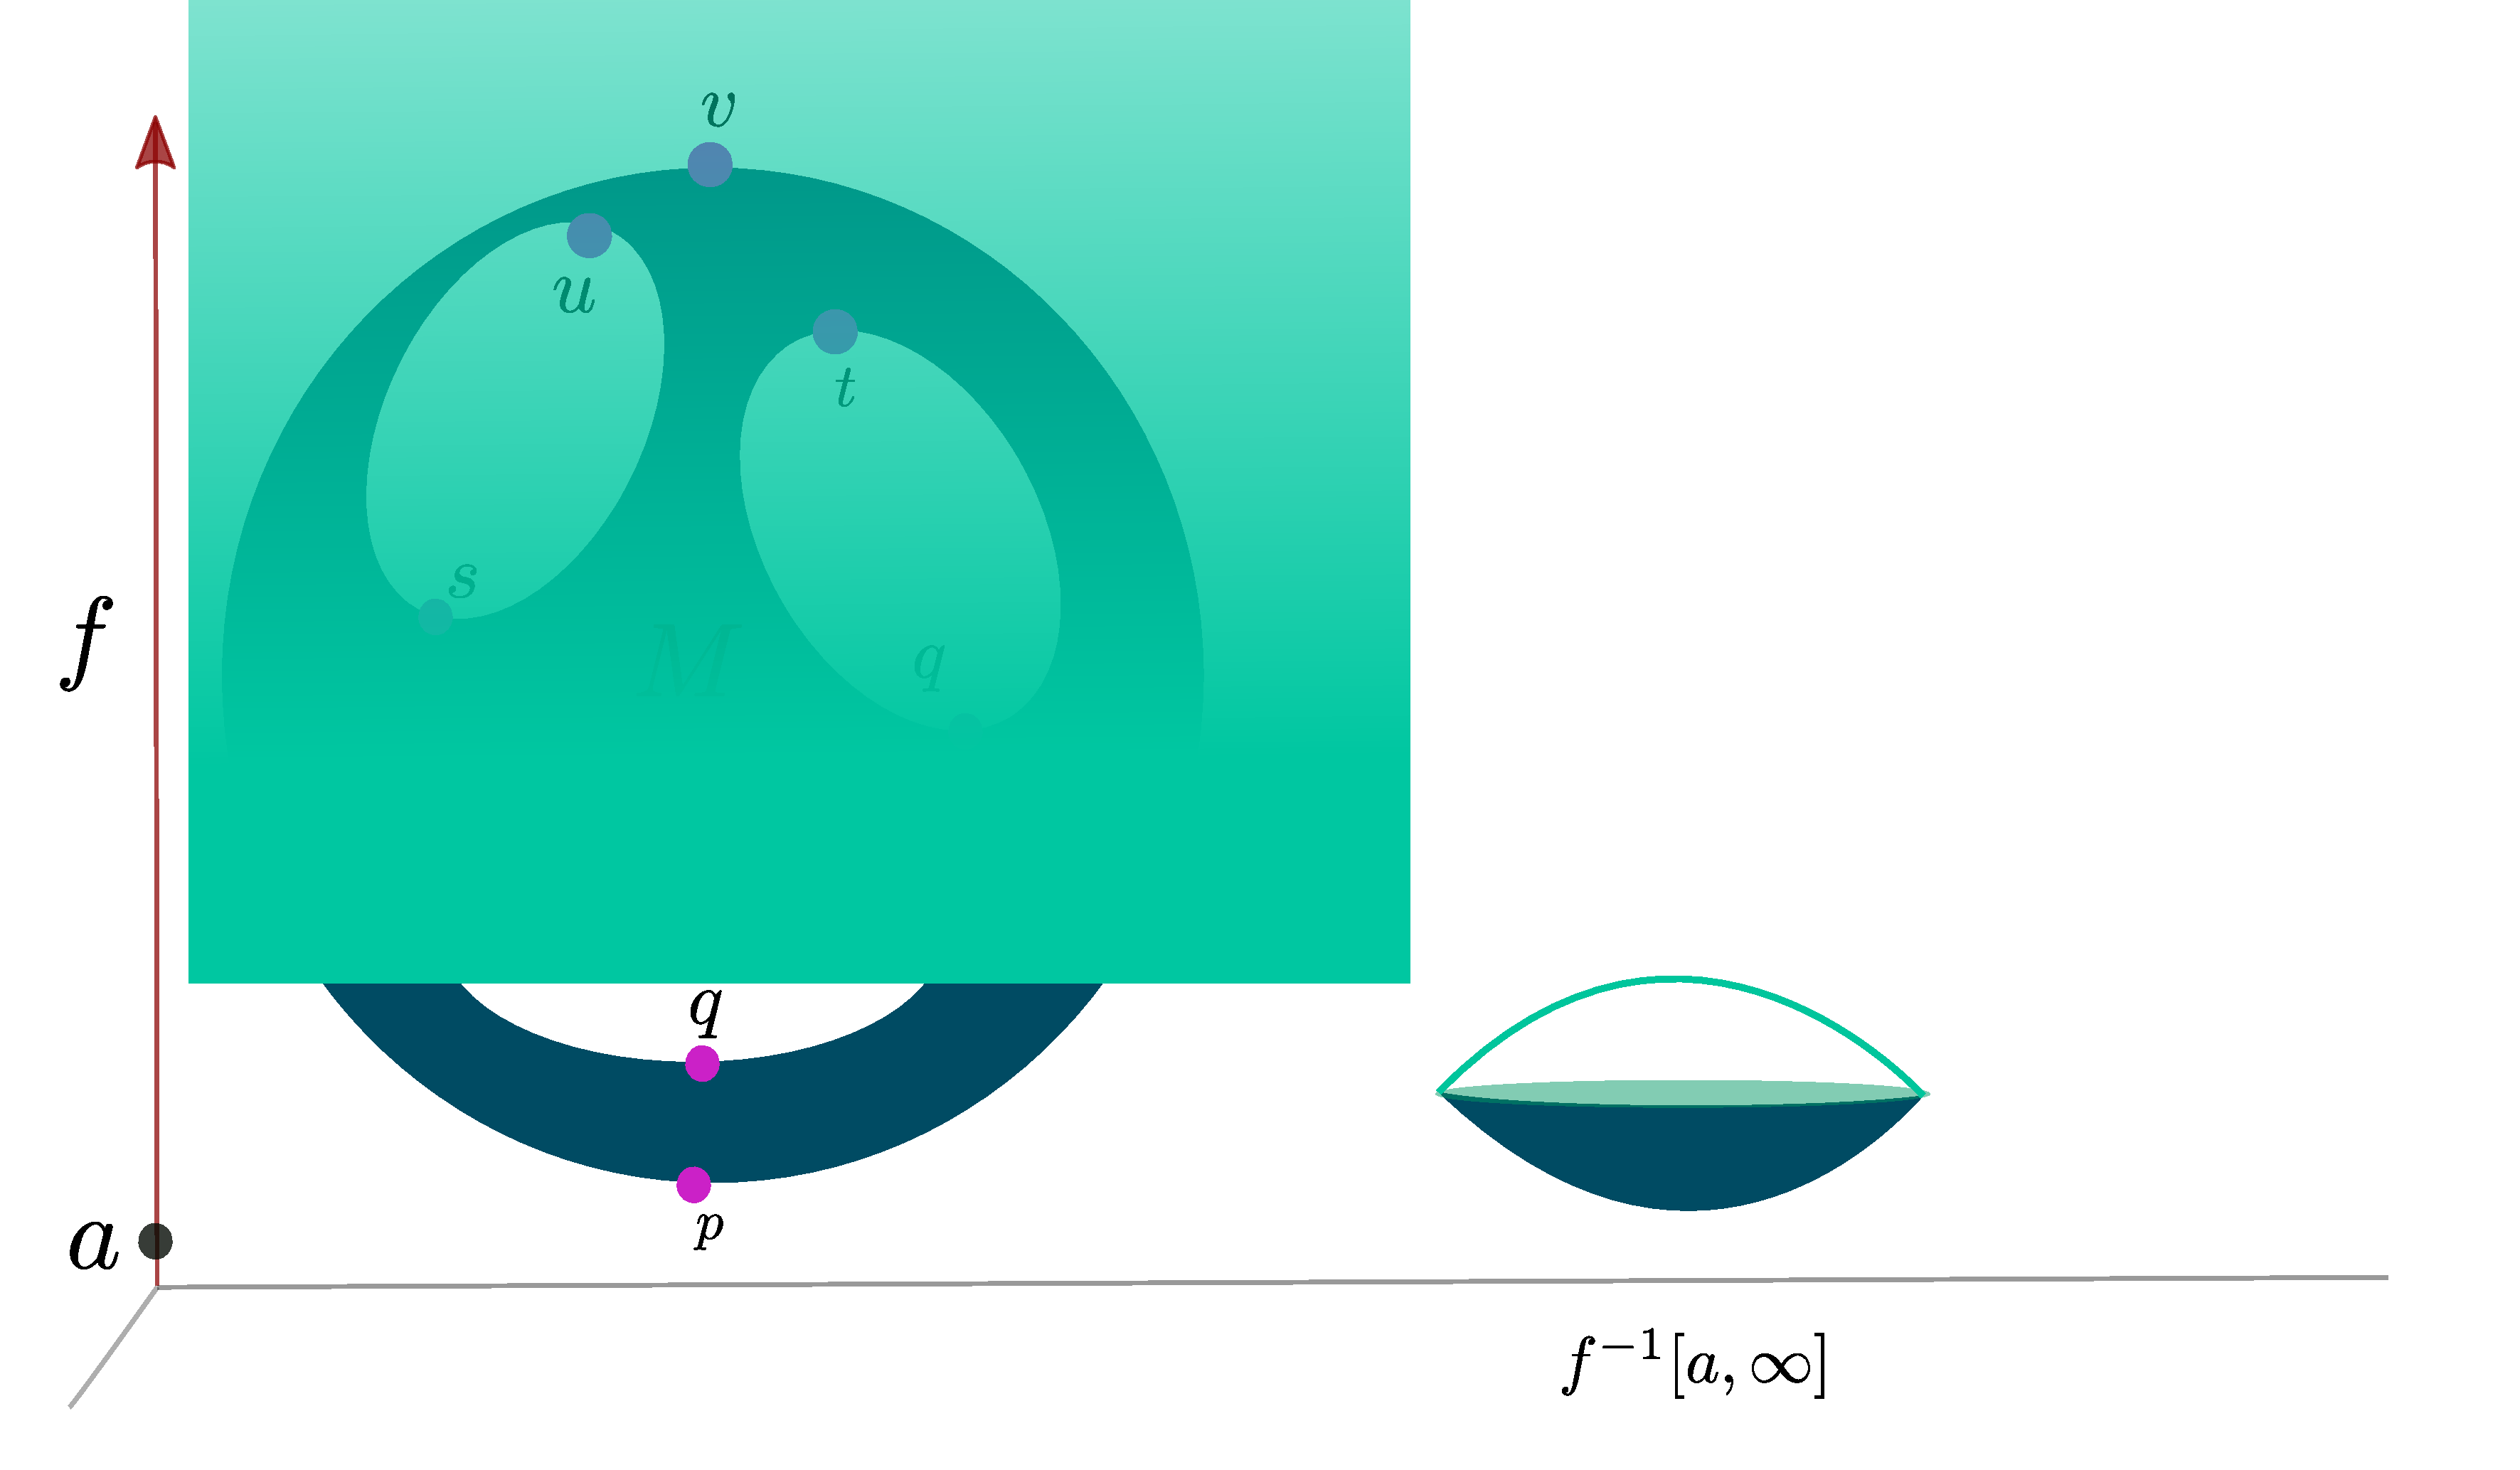
\includegraphics[scale=0.2]{3}
    \caption{Sub-level Set}
  \end{figure}
\end{frame}

\begin{frame}{Classical Morse Theory}
  \begin{figure}
    \centering
    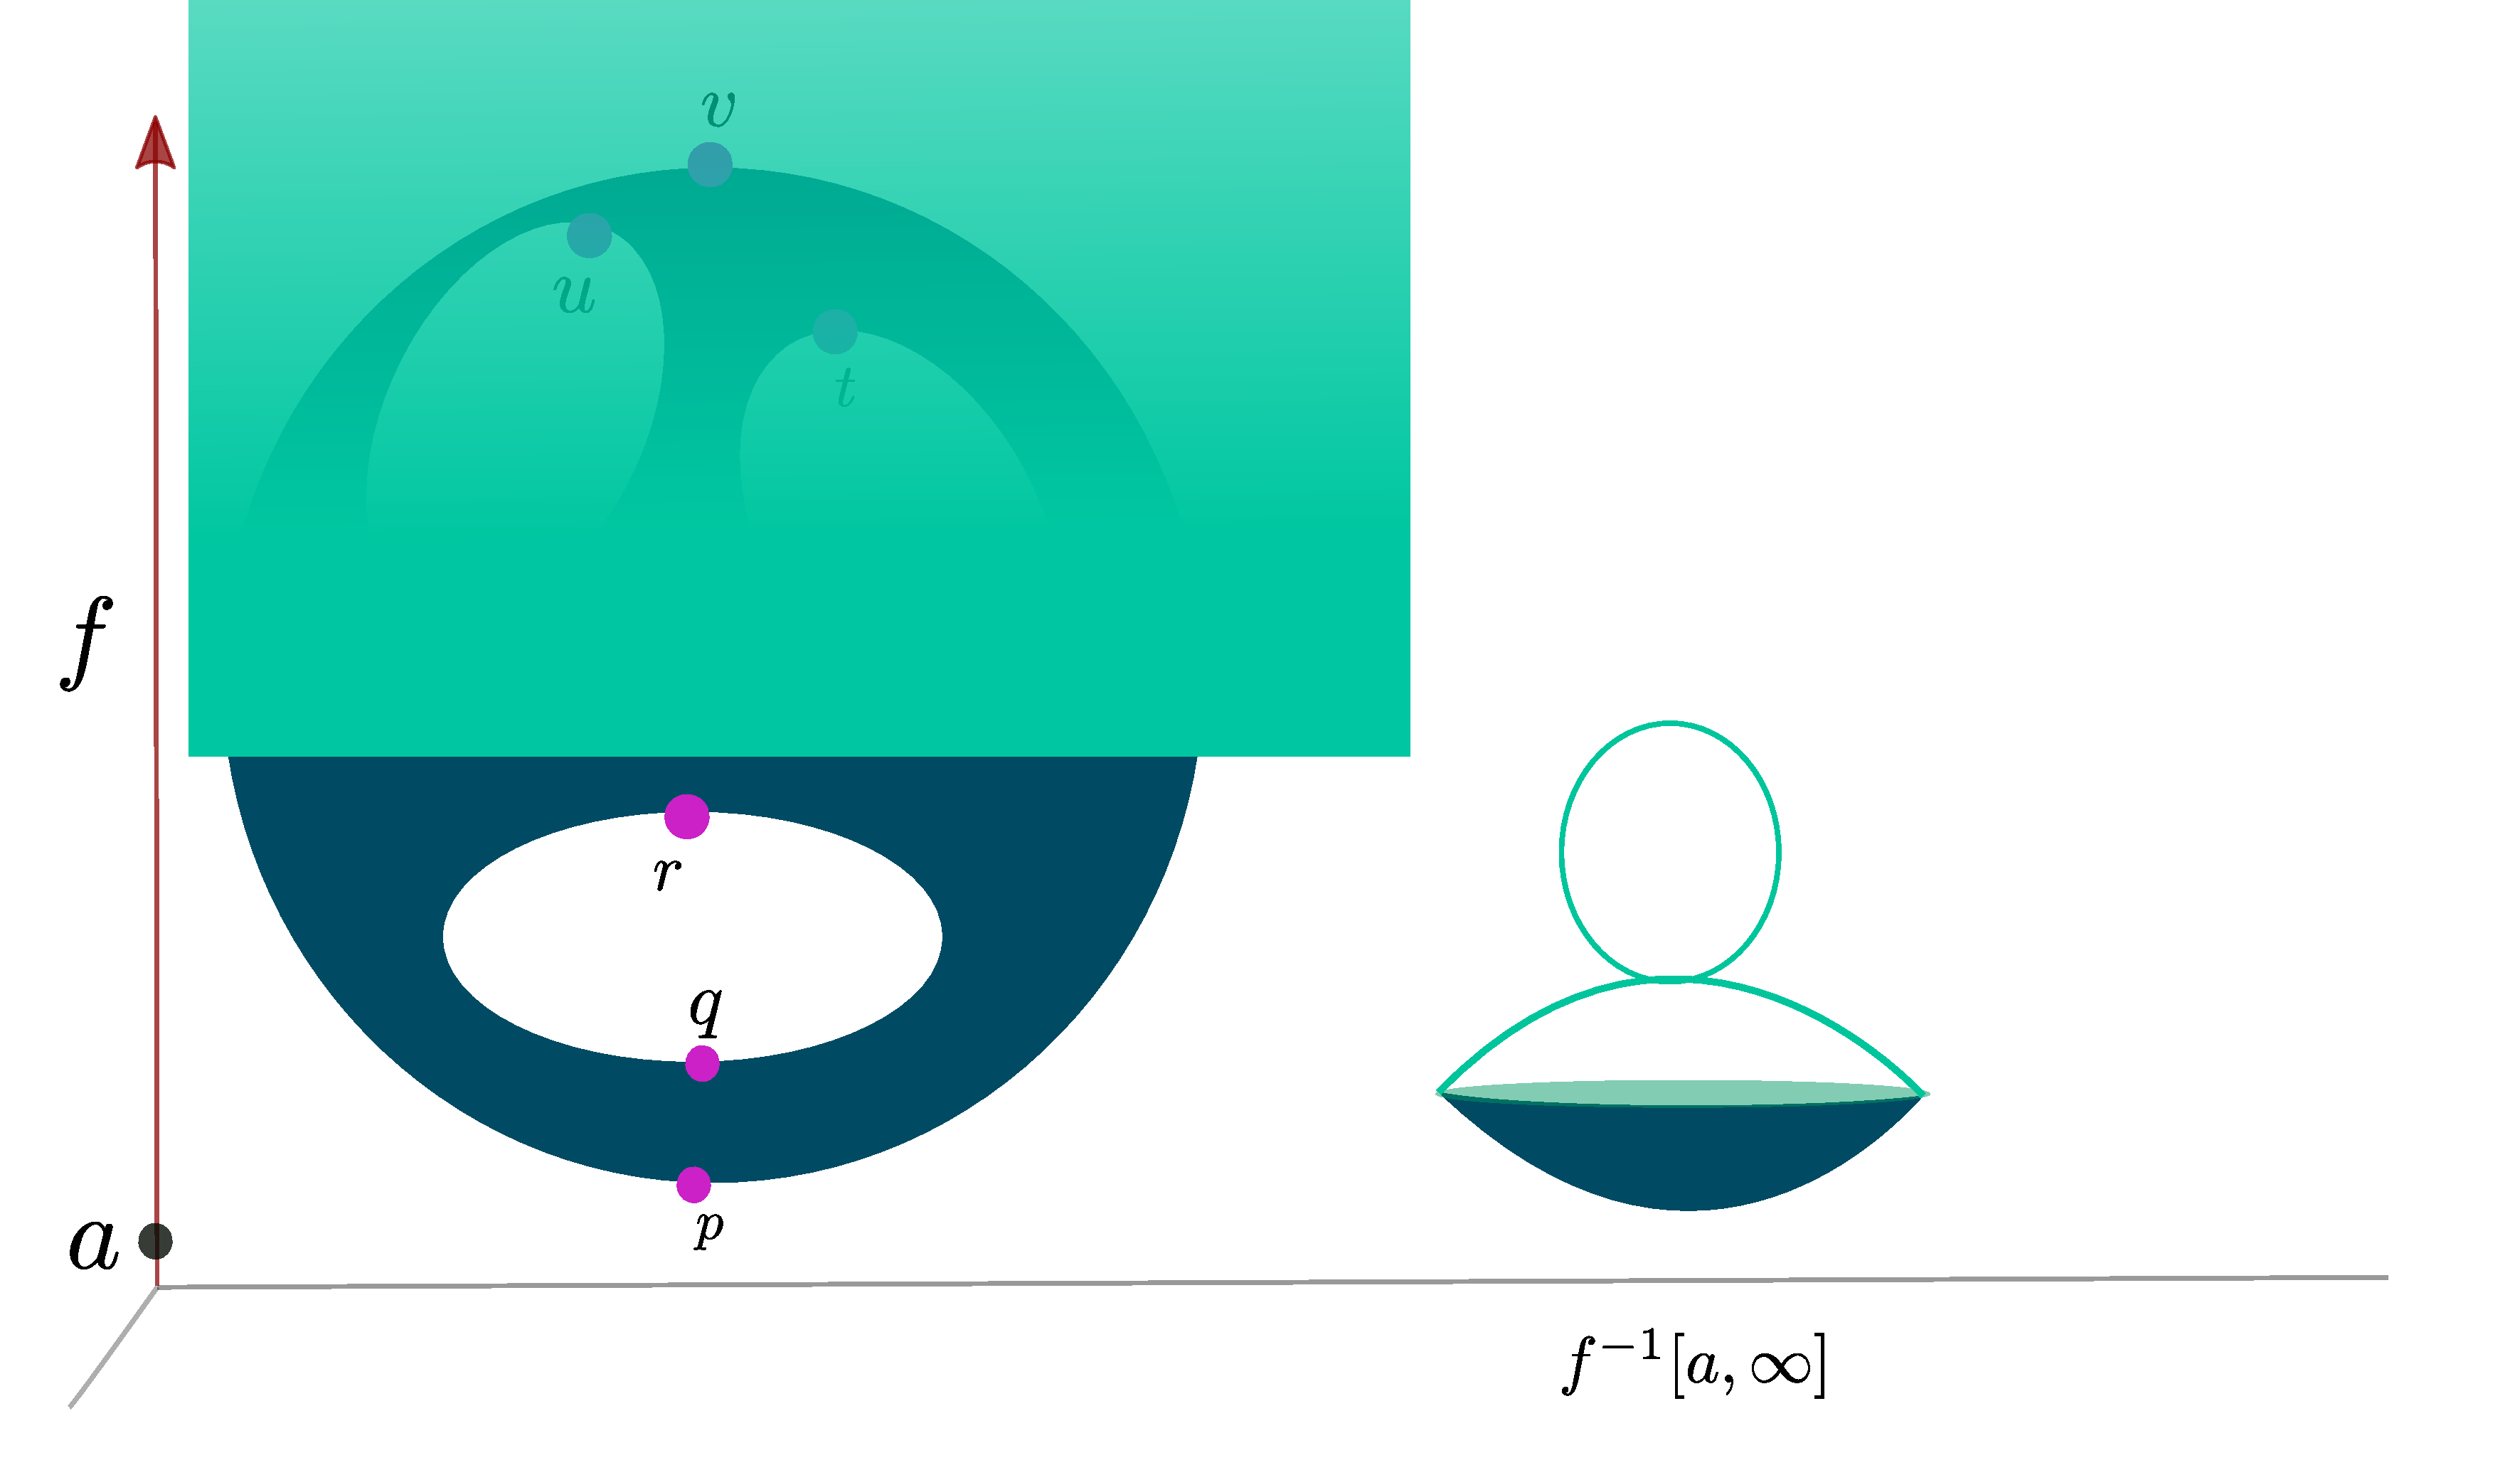
\includegraphics[scale=0.2]{4}
    \caption{Sub-level Set}
  \end{figure}
\end{frame}

\begin{frame}{Classical Morse Theory}
  \begin{figure}
    \centering
    
\includegraphics[scale=0.2]{5}
    \caption{Morse Complex}
  \end{figure}
\end{frame}

\begin{frame}{Classical Morse Theory}
  \begin{block}{Morse Theorem}
    If $f$ is Morse on $M$, then $M$ is \emph{homotopy equivalent} to a
    CW-complex having a $d$-cell for each critical point of $f$ of index $d$.
  \end{block}

  \pause
  
  \begin{block}{Morse Inequality}
    \#~critical $d$-index critical points $\geq H_d(M)$.
  \end{block}
\end{frame}


\begin{frame}{Dynamics of Morse Functions}
  \begin{block}{Gradient of Morse Function}  
    The gradient vector field of a smooth function $f$
    $$\langle\nabla f,V\rangle:=-Df(V),$$
    for any other vector field $V$ on $M$.
  \end{block}

  \pause
  
  \begin{block}{Stable Manifold}
    The \textcolor{blue}{stable manifold} $$W_s(p)=\{x\in
    M\mid\lim_{t\to\infty}\Phi_t(x)=p\}$$
  \end{block}

  \pause
  
  \begin{block}{Unstable Manifold}
    The \textcolor{blue}{unstable manifold} $$W_s(p)=\{x\in
    M\mid\lim_{t\to-\infty}\Phi_t(x)=p\}$$
  \end{block}  
  
\end{frame}

\begin{frame}{Dynamics of Morse Functions}
  \begin{block}{Observations}
    For a Morse function $f$ on a compact manifold $M$,
    \begin{enumerate}
    \item critical points are the equilibrium points of $\nabla f$.
      \pause
    \item $f$ (strictly) decreases along the flow-lines. 
      \pause
    \item no limit cycles.
    \end{enumerate}
  \end{block}
\end{frame}

\begin{frame}{Application}
  \begin{block}{Problem Statement}
    Given a (noisy) sample $S$ taken around a (hidden) embedded graph $G$, how
    one can ``\textcolor{blue}{reconstruct}'' the topology and geometry of $G$
    from $S$.
  \end{block}
  
  \begin{figure}[htb]
    \centering 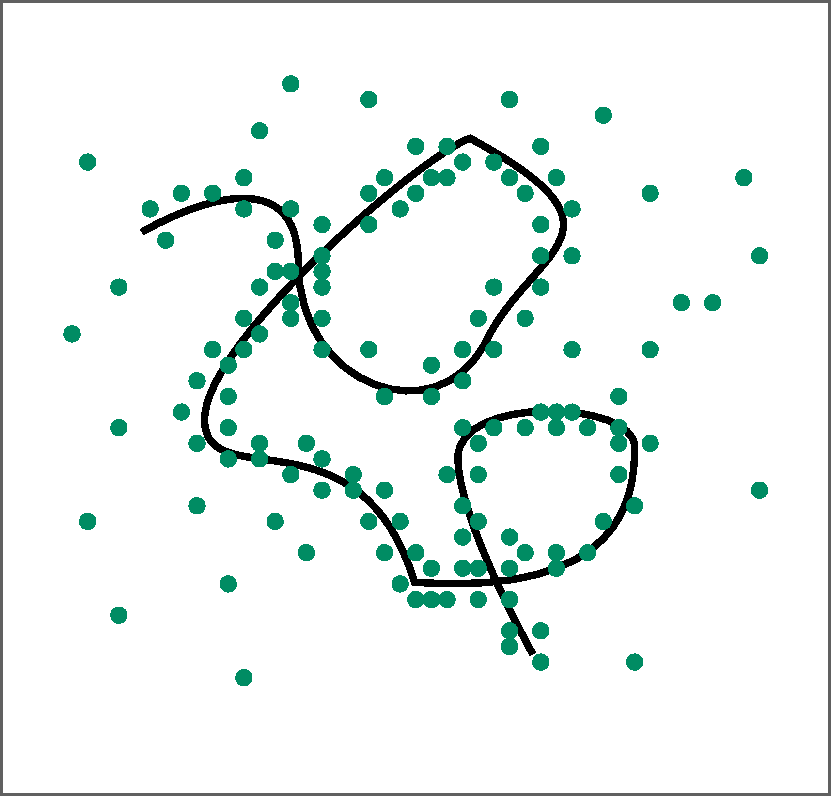
\includegraphics[scale=0.3]{sample}
    \caption{Sample around an embedded graph}
  \end{figure}
\end{frame}

\begin{frame}{Map Reconstruction from GPS traces}
  \begin{figure}[htb]
    \centering 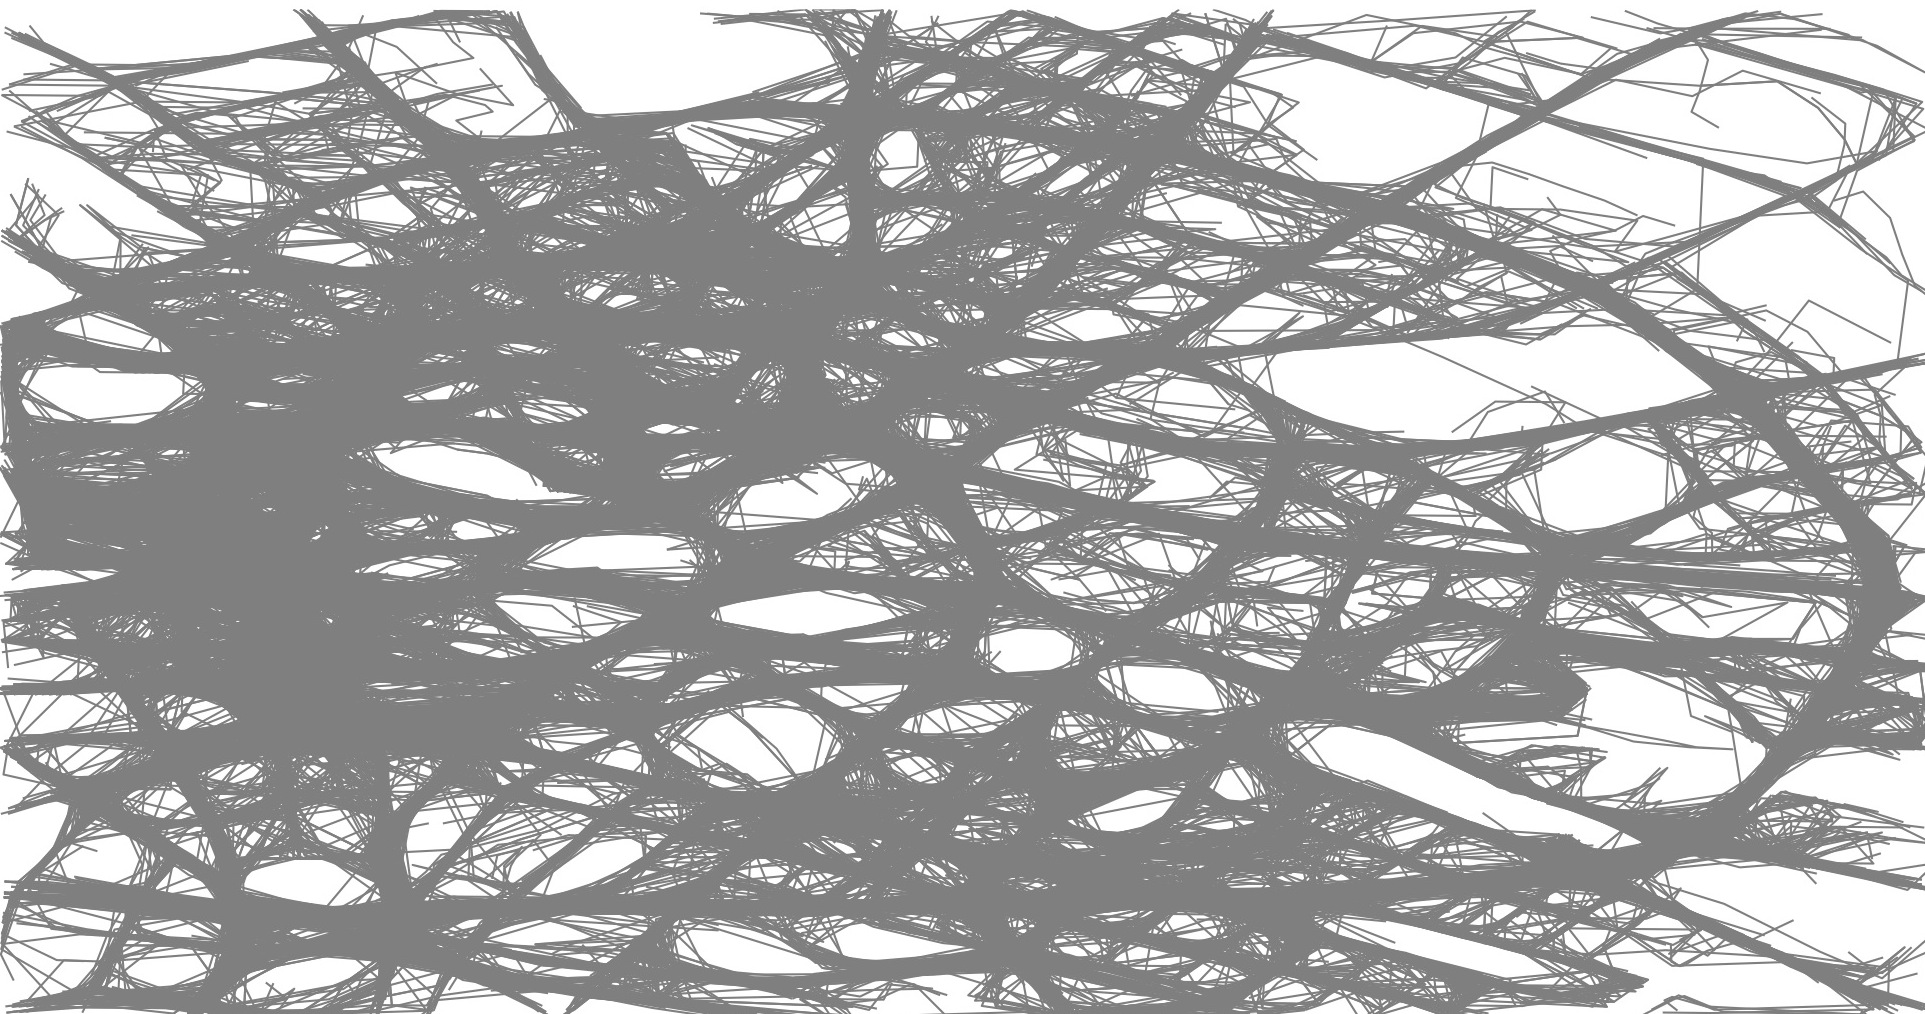
\includegraphics[scale=0.15]{Berlin}
    \caption{GPS traces of Berlin (mapreconstruction.org)}
  \end{figure}
  
  \pause
  \begin{figure}[htb]
    \centering 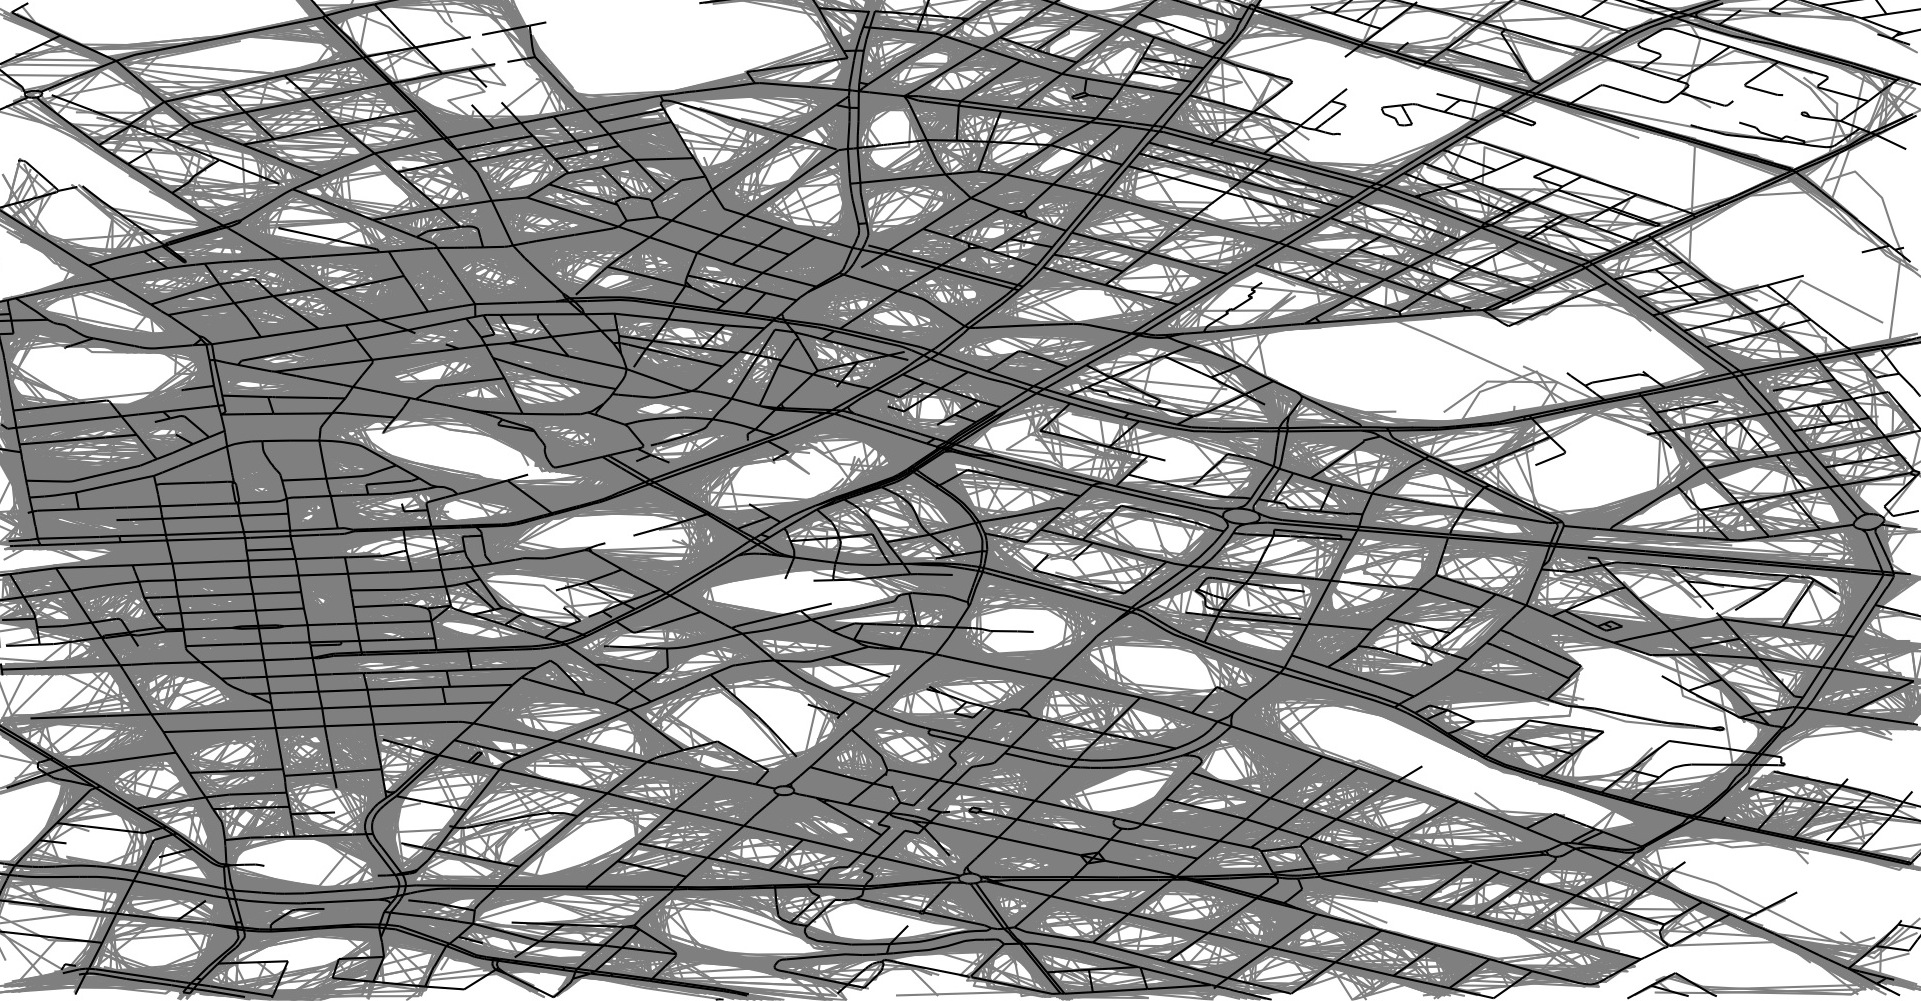
\includegraphics[scale=0.2]{Berlin_Recon}
    \caption{A reconstruction}
  \end{figure}
\end{frame}

\begin{frame}{Noise Models and Reconstruction}
  \begin{block}{Noise Models}
    \begin{enumerate}
    \item Hausdorff noise
      \pause
    \item Non-Hausdorff noise
    \end{enumerate}
  \end{block}
  
  \pause
  
  \begin{block}{What to reconstruct?}
    \begin{enumerate}
    \item Topology
      (\textcolor{blue}{homotopy type})
      \pause
    \item Geometry
      (\textcolor{blue}{Hausdorff-close})
      \pause
    \end{enumerate}
  \end{block}
\end{frame}


\begin{frame}{Density-Based Map Construction}
  \begin{block}{Generic Density-Based Algorithm}
    Given a discretized domain $\tilde D$ and a sample $S$ around $G$.
    \begin{enumerate}
    \item Compute density $f$ of $S$ over $\tilde D$. \\
      \pause
      \begin{itemize}
        \color{blue}
      \item
        {Histogram Computation}
        \pause
      \item Kernel Density Estimate
        $$K(x,y;\tau):=\exp\bigg(\frac{-\|x-y\|^2}{2\tau^2}\bigg)$$
        $$f(x)=\frac{1}{2\pi n\tau^2}\sum_{X_i\in S} K(x,X_i;\tau)$$
      \end{itemize}
      \pause
    \item for an appropriate threshold $t$, $f^{-1}[t,\infty)$ is considered.
      \pause
    \item heuristic pruning methods are applied this super-level set to
      approximate $G$.
    \end{enumerate}
  \end{block}
\end{frame}

\begin{frame}{Related Work}
  \begin{block}{Recent Works}
    \begin{enumerate}
    \item Choosing thresholds systematically using
      \textcolor{blue}{Persistent Homology}.
      Ahmed, Fasy et al. \cite{Ahmed:2015:CTD:2820783.2820810}
      \pause
    \item Graph reconstruction by \textcolor{blue}{Discrete Morse theory}.
      Dey, Wang et al.\cite{dey_graph_2018_socg}
    \end{enumerate}
  \end{block}

  \pause
  
  \begin{block}{Limitations}
    \begin{enumerate}
    \item Thresholds are chosen heuristically.
      \pause
    \item Theoretical guarantees on the topological/geometric correctness is not
      proved.
      \pause
    \item The output is often a thick region around the hidden graph.
    \end{enumerate}
  \end{block}
\end{frame}

\begin{frame}{Back to Morse}
  \begin{figure}[htb]
    \centering 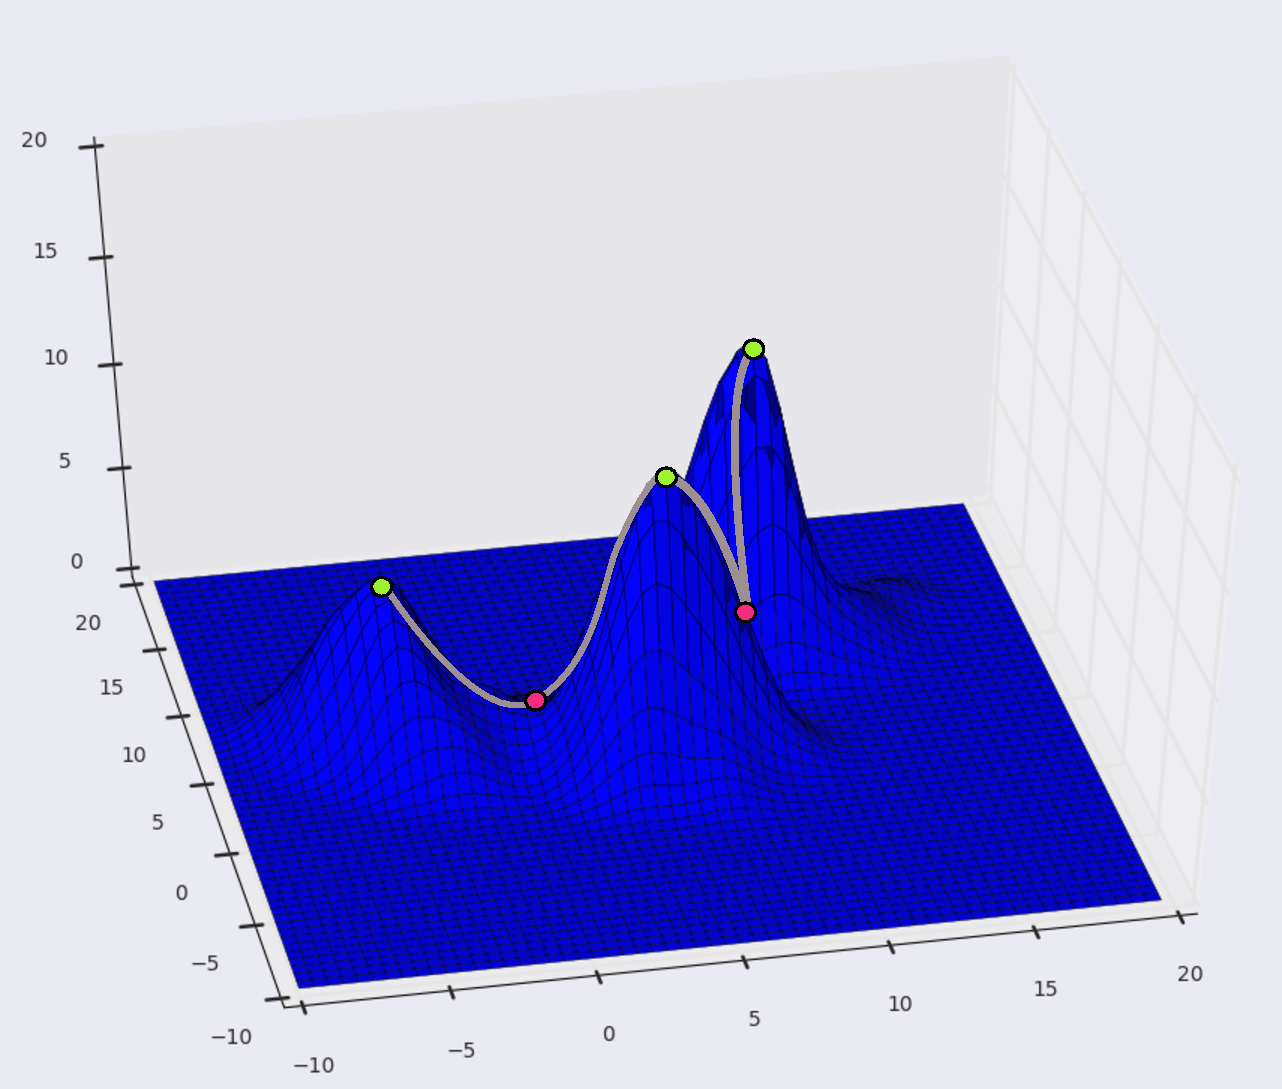
\includegraphics[scale=0.27]{ridges}
    \caption{KDE}
  \end{figure}

  \begin{block}{}
    If the samples are concentrated around a graph, then the mountain ridges on
    the graph of the density function are expected to capture it.
  \end{block}
\end{frame}

\begin{frame}{Discrete Morse Theory}
  \begin{block}{Discrete Morse Function}
    Let $K$ be a simplicial complex. A function $f:K\to\mathbb R$ is a
    \textcolor{blue}{discrete Morse function} if for every $\alpha^{(p)}\in K$
    \begin{enumerate}
    \item $\#\{\beta^{(p+1)}>\alpha | f(\beta)\leq   f(\alpha)\}\leq 1,$
    \item $\#\{\gamma^{(p-1)}<\alpha | f(\gamma)\geq f(\alpha)\}\leq 1.$ 
    \end{enumerate}
  \end{block}
  
  \pause
  
  \begin{figure}[htb]
    \centering 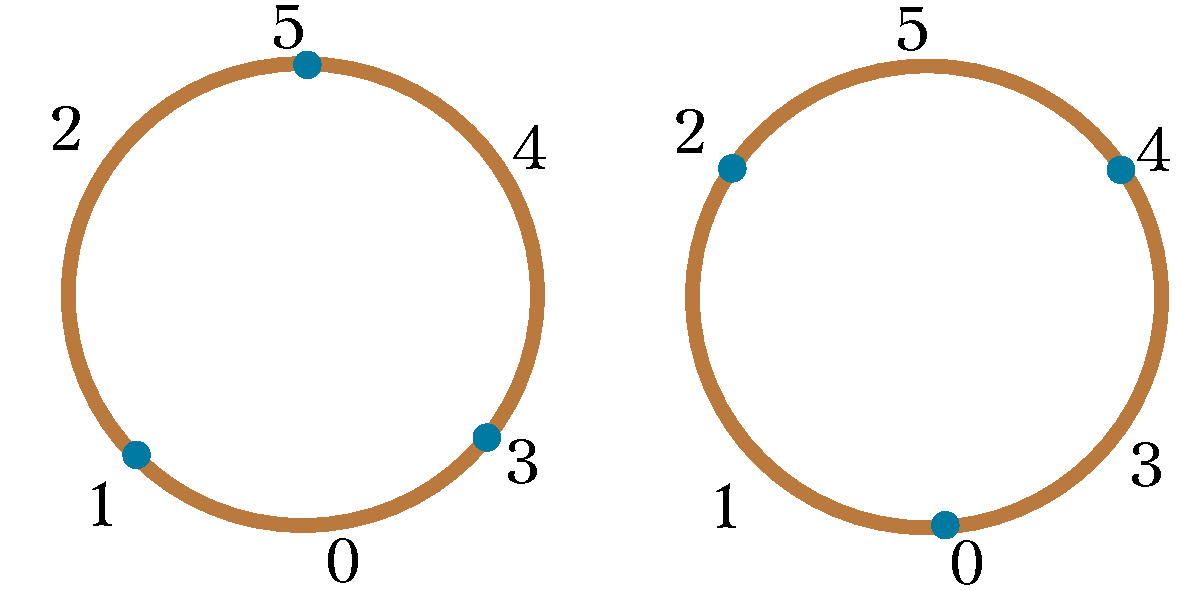
\includegraphics[scale=0.5]{discreteMorse}
    \caption{Discrete Morse Function}
  \end{figure}
  
\end{frame}


\begin{frame}{Discrete Morse Theory}
  \begin{block}{Critical Simplex}
    A simplex $\alpha^{(p)}$ is critical if
    \begin{enumerate}
    \item $\#\{\beta^{(p+1)}>\alpha | f(\beta)\leq   f(\alpha)\}=0,$
    \item $\#\{\gamma^{(p-1)}<\alpha | f(\gamma)\geq f(\alpha)\}=0.$ 
    \end{enumerate}
  \end{block}
  
  \pause
  
  \begin{figure}[htb]
    \centering 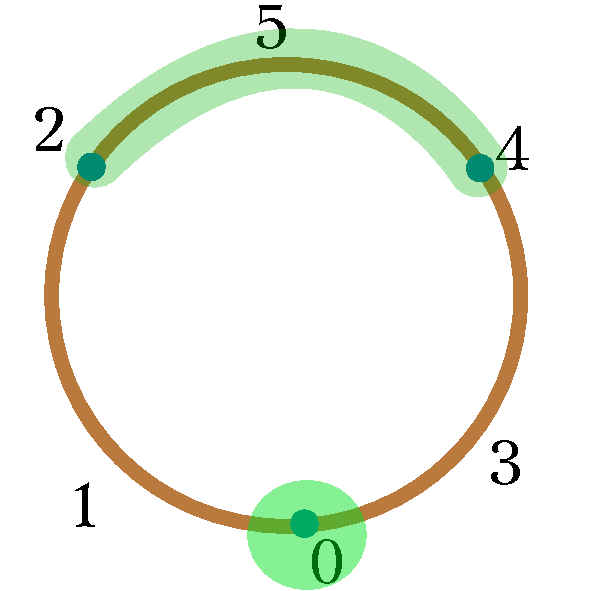
\includegraphics[scale=0.5]{discreteCritical}
    \caption{Discrete Morse Function}
  \end{figure}
  
\end{frame}

\begin{frame}{Discrete Morse Theory}
  \begin{block}{Discrete Morse Theorem}
    $K$ is a simplicial complex with a discrete Morse function. Then $K$ is
    homotopy equivalent to a CW-complex with exactly one cell of dimension $p$
    for each critical simplex of dimension $p$.
  \end{block}

  \pause
  
  \begin{figure}[htb]
    \centering 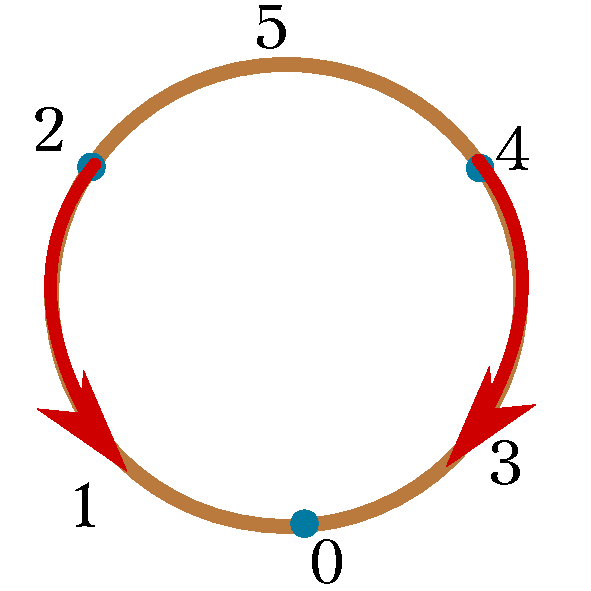
\includegraphics[scale=0.5]{vectors}
    \caption{Simplicial Collapse}
  \end{figure}
\end{frame}

\begin{frame}{Discrete Morse Theory}
 \begin{figure}[htb]
    \centering 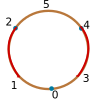
\includegraphics[scale=0.3]{vector}
    \caption{Simplicial Complex $K$ and discrete vector}
  \end{figure}

 \begin{block}{Discrete Vector Field}
   $(\sigma,\tau)$ is a \textcolor{blue}{discrete vector} in $K$ if
   $\tau<\sigma$. 
 \end{block}
\end{frame}

\begin{frame}{Discrete Morse Theory}
 \begin{figure}[htb]
    \centering 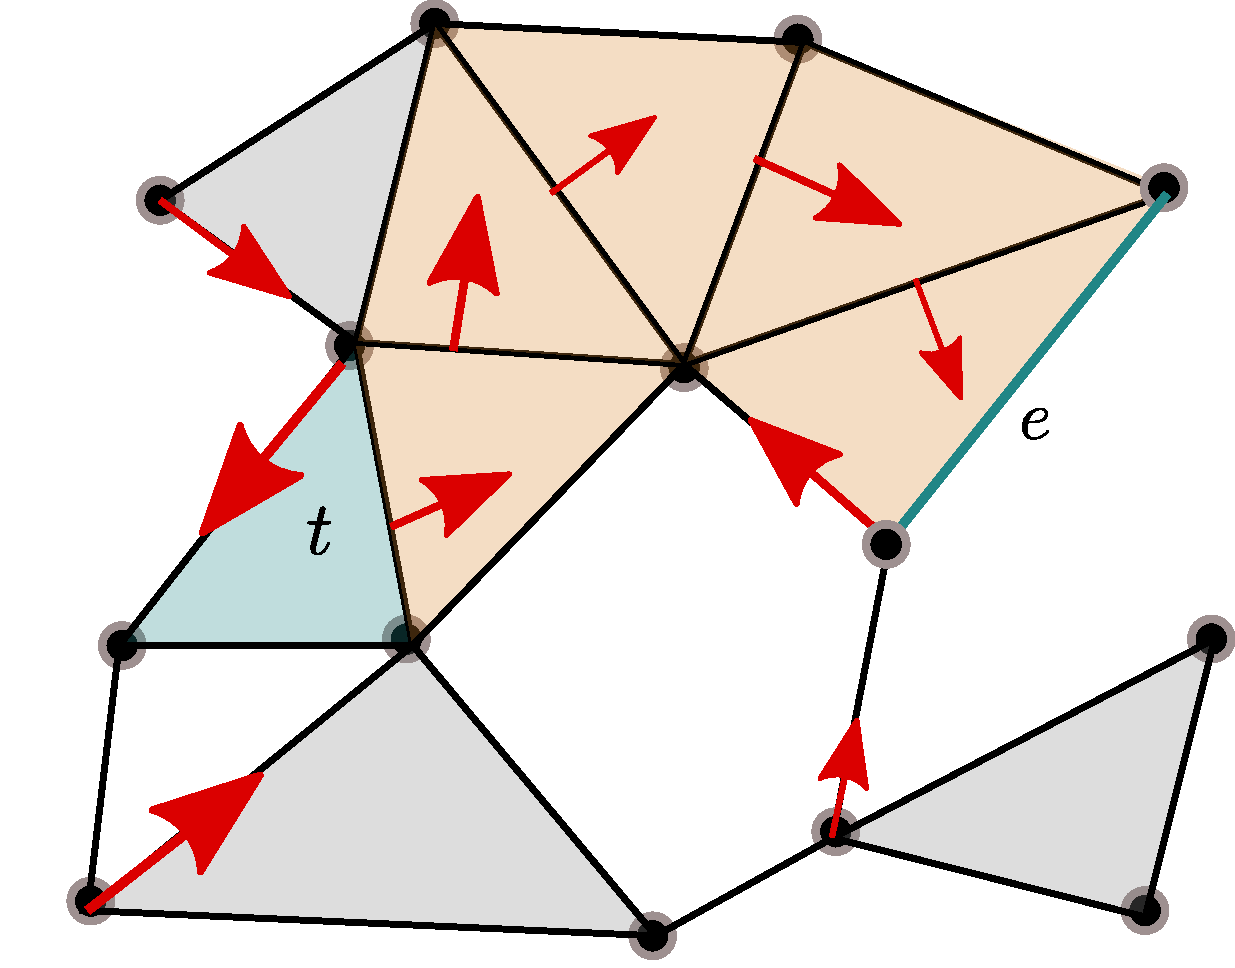
\includegraphics[scale=0.3]{vpath}
    \caption{Simplicial Complex $K$ and discrete vector}
  \end{figure}

 \begin{block}{Discrete Vector Field}
   $(\sigma,\tau)$ is a \textcolor{blue}{discrete vector} in $K$ if
   $\tau<\sigma$.  A discrete vector field is a collection of discrete vectors
   such that every simplex of $K$ is head/tail of at most one vector. 
 \end{block}
\end{frame}


\begin{frame}{Background: Discrete Morse Theory}
 \begin{figure}[htb]
    \centering 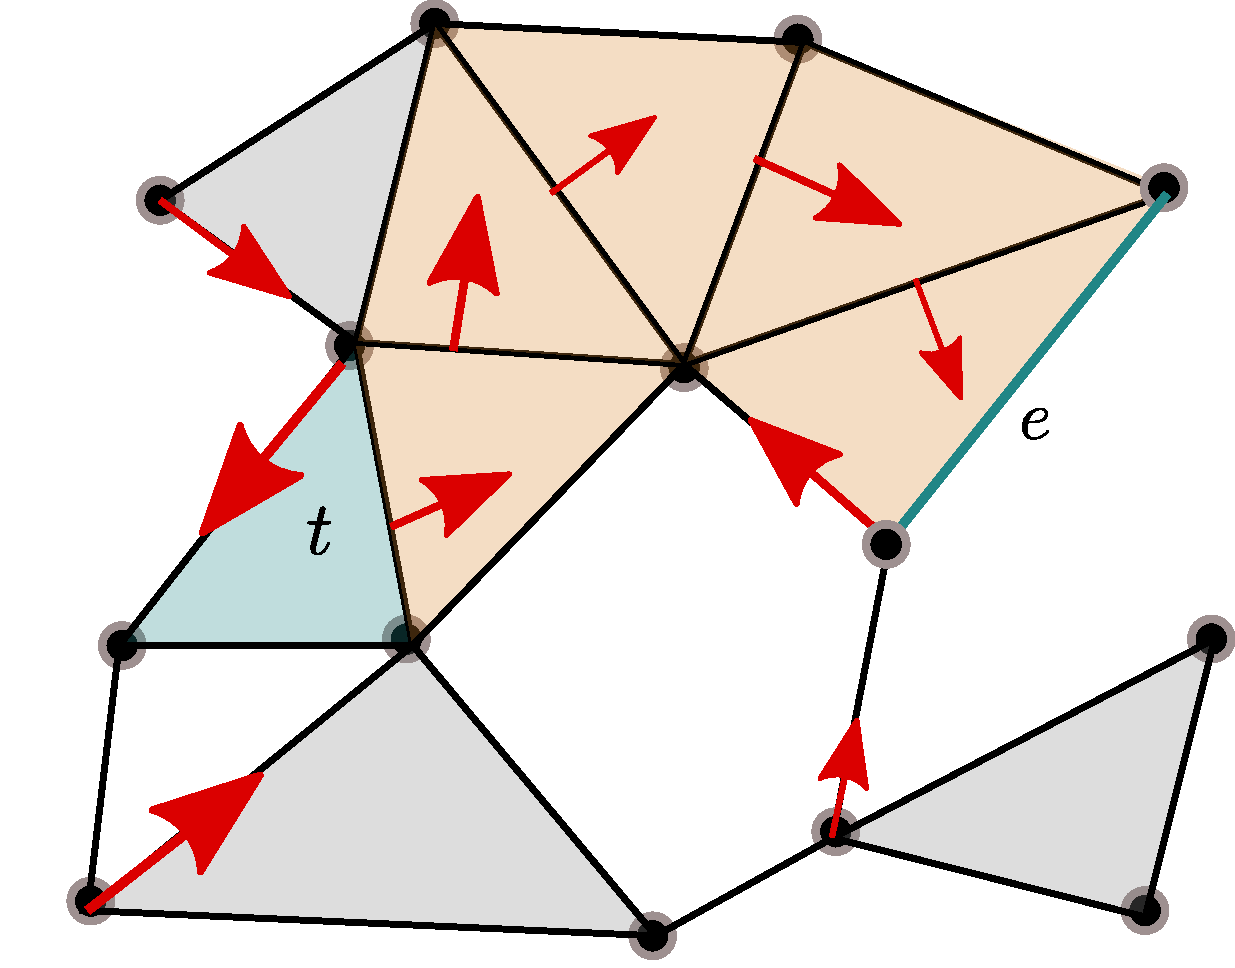
\includegraphics[scale=0.3]{vpath}
    \caption{V-path}
  \end{figure}

 \begin{block}{V-path}
   $$\sigma_0,\tau_0,\sigma_1,\tau_1,\ldots,\sigma_{l+1}$$
   where $(\sigma_i,\tau_i)$ is a vector and $\tau_i<\sigma_{i+1}$.
 \end{block}
\end{frame}

\begin{frame}{Background: Morse Cancellation}
  \begin{figure}[htb]
    \centering 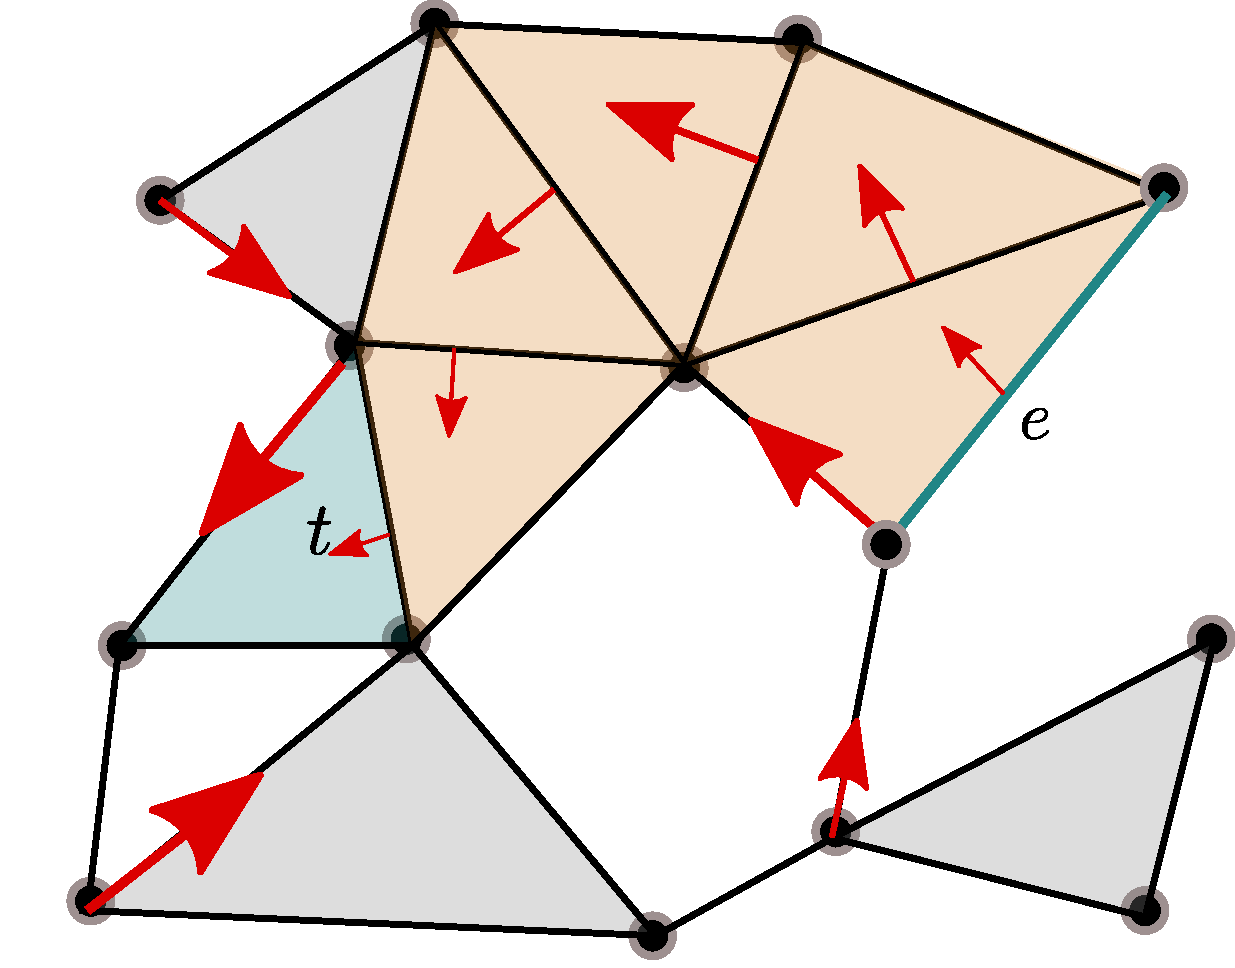
\includegraphics[scale=0.3]{cancellation}
    \caption{Morse Cancellation}
  \end{figure}

  \pause
  
  \begin{block}{Stable Manifold}
    For a critical edge $e$, its \textcolor{blue}{stable manifold} is the set of
    all V-paths ending at the boundary of $e$.
  \end{block}
\end{frame}

\begin{frame}{Assumption on the Density Function}
  \begin{block}{$(\omega,\beta_1,\beta_2,\nu)$-approximation of $G$}
    \[
    f(x)\in
    \begin{cases}
      [\beta_1, \beta_1+\nu],&  x\in V^\omega \\
      [\beta_2, \beta_2+\nu],&  x\in E^\omega \\
      [0,\nu],& \text{ otherwise }
    \end{cases}
    \]
  \end{block}
\end{frame}

\begin{frame}{Our Algorithm}
  Input: The discretized domain $K$, the density function $f$, the threshold
  $\delta$ \\
  Output: The reconstructed graph $\hat G$
  \begin{enumerate}
  \item Initialize $V$ as the trivial vector field on $K$ and $\hat{G}=\emptyset$.
  \item Run persistence on the super-level set filtration of $f$ to get the
    persistence pairs $P(K)$.
  \item For each $(\sigma,\tau)\in P(K)$ with $Pers(\sigma,\tau)<\delta$ \\ Try
    to perform a Morse cancellation for the pair and update V.
  \item For each $(v,e)\in P(K)$ and $(e,t)\in P(K)$ with $Pers(v)\geq\delta$,
    $\hat G$ = $\hat G\cup\{\text{ stable manifold of } e\}$.
  \item   output $\hat G$
  \end{enumerate}    
\end{frame}

\begin{frame}{Our Result}

  \begin{theorem}{}
    If $G$ is a connected, embedded planar graph in a cubical complex $K$ and
    $f$ is an $(\omega,\beta_1,\beta_2,\nu)$-approximation then the output $\hat
    G$ has the same homotopy type as $G$. Moreover, $d_H(G,\hat G)<\omega$.
  \end{theorem}
\end{frame}

  
\begin{frame}{Future Work}
  
  \begin{enumerate}
  \item How to circumvent the heavy persistence computation.
    \pause
  \item What condition on the density function gives up a small Fr\'echet
    distance between the edges of the output and the edges of the graph.  \pause
  \item Extend the result to higher dimensions.
  \end{enumerate}
\end{frame}

\begin{frame}
  \centering
  \Huge{\textcolor{magenta}{Thanks}}
\end{frame}

\begin{frame}[allowframebreaks]
        \frametitle{References}
        \bibliographystyle{amsalpha}
        \bibliography{bib}
\end{frame}
\end{document}
